\chapter{Stand van zaken}
\label{ch:stand-van-zaken}

% Tip: Begin elk hoofdstuk met een paragraaf inleiding die beschrijft hoe
% dit hoofdstuk past binnen het geheel van de bachelorproef. Geef in het
% bijzonder aan wat de link is met het vorige en volgende hoofdstuk.

% Pas na deze inleidende paragraaf komt de eerste sectiehoofding.


In dit hoofdstuk zal er een stand van zaken gegeven worden van het onderwerp, hoe het vroeger gebeurde en hoe het tegenwoordig gebeurt. Eerst en vooral zal sectie \ref{sec:HCE} wat meer uitleg geven over HCE en hoe het simuleren van draadloze smart cards gebeurt. In sectie \ref{sec:NFC} zal een korte uitleg gegeven worden over NFC technologie. Sectie \ref{sec:SE} geeft een betere kijk op wat een Secure Element (SE) is. Sectie \ref{sec:Bedreigingen} toont een aantal bedreigingen voor contactloze betalingsappplicaties. In sectie \ref{sec:hardwareEnRisico} hoe beveiliging op hardware niveau werkt vs risicobeperking. Ten slotte zal in sectie \ref{sec:Beveiliging} uitgelegd worden welke manieren er bestaan om HCE te beveiligen.


\section{Host-based Card Emulation (HCE)}
\label{sec:HCE}
Sinds de komst van Android 4.4 oftewel Android KitKat introduceerde Google een nieuwe technologie genaamd Host-based Card Emulation (HCE). HCE technologie maakt het mogelijk om Near Field Communication (NFC) technologie te gebruiken zonder de aanwezigheid van een secure element. De nood voor deze technologie is er gekomen door de sterke afhankelijkheid aan de producent die bij het gebruik van een secure element erbij komt. Ook niet ieder mobiel toestel beschikt over een secure element hierdoor was er geen één oplossing voor alle toestellen mogelijk. HCE is beschikbaar vanaf Android4.4, dit betekent dat meer dan 90\% van de actieve android toestellen instaat zijn om gebruik te maken van host-based card emulation technologie. Wanneer het Android toestel zich in card emulation (CE) mode bevindt en tegen een draadloze lezer of point-of-sale (POS) terminal gehouden wordt, heeft het toestel de mogelijkheid om allerhande soorten draadloze smart cards te simuleren. Deze contactloze smart cards worden in vele situaties gebruikt zoals bij draadloos betalen, loyalty systemen, ticketing, toegang tot gebouwen ... ~\autocite{SCA2014}.

HCE maakt het dus mogelijk voor NFC-apparaten om draadloze smart cards te simuleren. Om gebruik te kunnen maken van HCE heeft Android verschillende libraries en APIs (Application Programming Interface) geïmplementeerd in het besturingssysteem. Deze libraries en APIs worden overschreven door de applicaties die hier gebruik van willen maken en die op de CPU van het apparaat draaien. Deze applicaties kunnen dan APDU (Application Protocol Data Unit) commando's en antwoorden uitwisselen met een NFC POS. Wanneer men vroeger gebruik wilde maken van de NFC technologie kon dit alleen door een Secure Element (SE) die ingebouwd zat in het apparaat zoals een SIM-kaart. De applicaties werden geïnstalleerd op deze SE die dan de APDU's afhandelde om zo draadloze smart cards veilig te kunnen simuleren. De APDU's die verstuurd worden van een NFC-lezer worden opgevangen door de NFC-antenne van het apparaat en wordt doorgegeven via de NFC controller naar het SE en omgekeerd (zie figuur  ~\ref{fig:SE-HCE}). Met HCE is het de bedoeling dat de nood van een SE verwijderd wordt uit deze operatie, in plaats van de APDU's door te geven naar het SE worden deze doorgegeven naar de CPU van het apparaat en omgekeerd (zie figuur ~\ref{fig:SE-HCE}) ~\autocite{Alattar2014}. 

\begin{figure}
	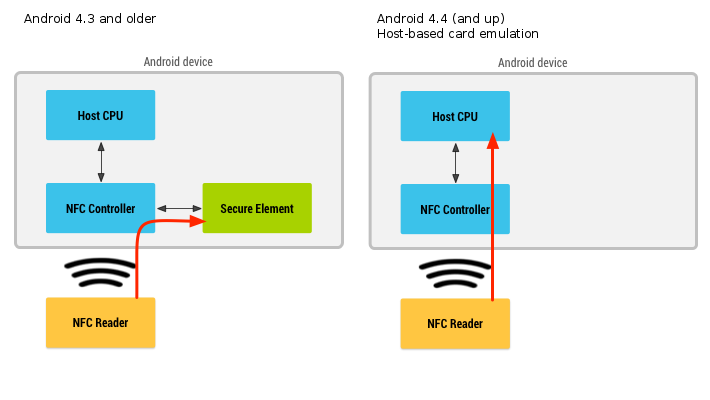
\includegraphics[width=\linewidth]
	{img/WalletHostBasedCardEmulation}
	\caption{Simulatie van een smart card via SE}
	\label{fig:SE-HCE}
\end{figure}


\section{Near Field Communication (NFC)}
\label{sec:NFC}
Near Field Communication (NFC) is een technologie die communicatie vanop korte afstanden, meestal nul tot vier centimeter maar kan tot 20 centimeter oplopen, mogelijk maakt. NFC apparaten kunnen actief of passief zijn, wanneer het NFC apparaat actief is dan gebruikt dit apparaat zijn eigen energiebron om zijn radio frequentie te genereren. Een passief NFC apparaat gebruikt de energiebron van een actief NFC apparaat om data te versturen, passieve NFC apparaten kunnen ook enkel maar antwoorden op aanvragen die vanaf een actief NFC apparaat verstuurd wordt. Transacties worden automatisch gestart door twee NFC apparaten elkaar te laten raken of deze twee dicht bij elkaar te houden ~\autocite{Alattar2014}. 

NFC heeft drie verschillende operating modes: Peer to Peer mode, Reader/Writer mode en Contactless Card Emulation. Peer To Peer mode biedt de mogelijkheid om data te versturen tussen twee NFC apparaten aan snelheden tot 424 Kbit/s. Reader/Writer mode maakt het mogelijk dat twee NFC apparaten gebruikt kunnen worden voor het lezen/schrijven van tags en draadloze smart cards, hierbij is de snelheid van het versturen van de data maar 106 Kbit/s. Contactless Card Emulation laat de NFC apparaten draadloze smart cards of tags simuleren die gelezen of naar geschreven kunnen worden door een NFC lezer ~\autocite{Alattar2014}. 


\section{Secure Element (SE)}
\label{sec:SE}
Een Secure Element is een hardware element binnenin een Android apparaat. Het doel van het Secure Element is om applicaties en al hun data veilig op te slaan, het Secure Element is hardwarematig beveiligd dus zorgt het voor de ideale plaats om de applicaties in op te slaan. Er bestaan drie verschillende soorten SE's: Universal Integrated Circuit Card (UICC), ingebouwde SE (eSE) en een microSD ~\autocite{Borko2014}. UICC is een meer geavanceerde vorm van een gewone SIM-kaart. ESE is een ingebouwde smart card die gesoldeerd is aan het moederbord van het apparaat. Ondanks dat een Secure Element één van de meest veilige manieren is om een applicatie en zijn data in op te slaan is het niet de gemakkelijkste. Niet ieder apparaat is in het bezit van een Secure Element. Dit zorgt er dus voor dat maar een klein aantal apparaten kunnen genieten van de voordelen van een Secure Element, iedere vorm van een Secure Element wordt ook beheerd door een andere producent wat het moeilijker maakt voor applicatieontwikkelaars om het SE te gebruiken. Door deze tekortkomingen kwam de nood voor Host-based Card Emulation technologie en de daarbij horende beveiliging voor HCE.


\section{Bedreigingen voor een contactloze betalingsapplicatie}
\label{sec:Bedreigingen}
De mogelijke bedreigingen voor mobiele applicaties veranderen voortdurend. Dit wetende moeten de ontwikkelers voor mobiele applicaties (in dit geval mobiele betalingsapplicaties) rekening houden met alle verschillende mogelijke bedreigingen en tegen maatregelen. Op de dag van vandaag is Host-based card emulation alleen maar beschikbaar op Android, er wordt verwacht dat Host-based card emulation overgebracht zal worden naar andere besturingssystemen zoals IOS en Windows. Het is dus belangrijk dat er in de toekomst security frameworks ontwikkeld worden die besturingssysteem onafhankelijk zijn, dit zorgt voor snelle en flexibele applicatie management ~\autocite{Cryptomathic}.

\subsection{Software Reverse Engineering}
Software Reverse Engineering (SRE) is het analyseren van software systemen in zijn geheel of een deel ervan om zo het ontwerp of implementatie informatie te ontdekken. Een typisch scenario waar SRE vaak gebruikt wordt is bij software waaraan al jaren is gewerkt en informatie over het bedrijf bevat in de geschreven code. Hackers kunnen gebruik maken van de verschillende standaard zwaktes van het besturingssysteem of protocollen samen met reverse engineering tools, scripting en op maat gemaakte software om zo informatie te verzamelen om hun aanval uit te voeren. Software ontwikkelaars overwegen best om hun software zo robuust mogelijk te maken zodat er veel tijd en innovatie nodig is van de hackers om een aanval te doen slagen ~\autocite{Cryptomathic}.

\subsection{Secure Data Storage}
Door gebruik te maken van Host-based card emulation en betalingstokens maakt het mogelijk voor de ontwikkelaars om onafhankelijk te werken van de grote bedrijven die de Secure Elements produceren. Dit zorgt er natuurlijk ook voor dat de gevoelige gegevens niet meer opgeslagen kunnen worden in een Secure Element wat het op zijn beurt weer gemakkelijker maakt voor hackers om deze data te verkrijgen. Hierdoor zal er een nieuwe oplossing moeten komen om de gevoelige data ergens veilig te kunnen opslaan waar de hackers niet gemakkelijk aan kunnen raken en ontmoedigd worden om een aanval te plegen ~\autocite{Cryptomathic}.

Secure data storage refereert naar data in rust toestand die opgeslagen wordt op computers, servers, harde schijven, draagbare toestellen zoals externe harde schijven en USB-sticks, online/cloud opslag, network-based storage area network (SAN) of network attached storage (NAS) systeem. Het veilig opslaan van de data op deze systemen kan bekomen worden door data encryption, access control, beveiliging tegen malware, fysieke beveiliging van opslagplaatsen, implementatie  van gelaagde opslag beveiliging architectuur.

\subsection{Malware}
Mobiele besturingssystemen hebben een heel ander beveiligings profiels in tegenstelling tot desktop besturingssystemen. Alle geïnstalleerde versies van een mobiel besturingssysteem moeten goedgekeurd worden door de producent van het besturingssysteem waardoor ze veiliger zijn. Ondanks de extra veiligheid wordt er vaak malware gevonden op mobiele systemen, de malware werkt altijd binnen de toegestane toestemmingen en kan dus geen al te grote schade aanrichten ~\autocite{Cryptomathic}.

Malware is een algemene naam die gebruikt wordt voor een groot aantal kwaadaardige software varianten zoals virussen, ransomware en spyware. Malware is code dat ontwikkeld is door cyber aanvallers met al doel grote schade aan te richten aan data en systemen of toegang te krijgen tot een netwerk. Malware wordt meestal verspreid  in de vorm van een link of bestand via email, de gebruiker moet klikken op de link of het bestand openen om de malware uit te voeren. Zoals eerder vernoemd zijn er verschillende soorten malware:

\begin{itemize}
	\item \textbf{Virus:} Een virus is de meest voorkomende vorm van malware. De kwaadaardige code die de virus met zich meebrengt wordt verborgen in de gewone code. Het virus wordt geactiveerd door een onwetende gebruiker of een geautomatiseerd proces. Een virus kan zich heel snel en ver verspreiden, het kan schade veroorzaken een de core functionaliteit van het systeem, bestanden onbruikbaar maken en gebruikers uit hun eigen computer sluiten.
	
	\item \textbf{Worms:} De worm heeft zijn naam gekregen door de manier waar de malware het systeem infecteert. De worm start op een machine en verspreidt zich over het netwerk om andere systemen te infecteren. Dit type malware kan snel een groot deel of zelfs alle systemen binnen een netwerk infecteren.
	
	\item \textbf{Spyware:} Spyware is ontwikkeld om te spioneren wat een gebruiker doet. De malware draait in de achtergrond van de computer en verzamelt informatie over de gebruiker zonder dat hij er weet van heeft. De informatie die spyware zoal kan verzamelen zijn bank gegevens, wachtwoorden en nog veel meer gevoelige informatie.
	
	\item \textbf{Trojans:} Trojans doen zich voor als legitieme software, de malware zal zich discreet gedragen en zal achterpoorten creëeren voor andere malware zodat ze het systeem kunnen binnendringen.
	
	\item \textbf{Ransomware:} Ransomeware kan een heel netwerk platleggen of een gebruiker uit zijn computer sluiten. De gebruiken moet een hoge dwangsom betalen om terug toegang te krijgen tot het netwerk of de computer. Ransomeware wordt veel gebruikt om grote organisaties aan te vallen en grote dwangsommen te ontvangen.
\end{itemize}

\subsection{Gebruik van een nep Point-of-Sale (POS)}
De point-of-sale heeft een belangrijke rol binnen het uitvoeren van een contactloze transactie en kan daardoor ook gebruikt worden door aanvallers om nieuwe transacties te starten of gevoelige bank data te onderscheppen. Wanneer een contactloze transactie gestart wordt genereert het mobiele toestel een contactloze transactie die verschillende parameters zoals het betalingstoken en verval datum bevat. Het mobiele toestel stuurt de gegevens naar de point-of-sale van de handelaar via de NFC interface. Een valse point-of-sale kan op veel verschillende manieren gecreëert worden door een aanvaller die slechte bedoelingen heeft:

\begin{itemize}
	\item \textbf{Externe nep POS:} Het gebruik van een extern toestel om te communiceren met de mobiele toestel van het slachtoffer via het NFC protocol. Wanneer zo een nep POS de communicatie flow correct implementeerd die gebruikt wordt door een echte POS, kan de aanvalleren communiceren met het mobiele toestel van het slachtoffer zonder dat de persoon het door heeft dat hij communiceert met een nep POS.
	
	\item \textbf{Interne nep POS:} Het gebruik van een applicatie die rechtstreeks kan communiceren met de API van de NFC controller via het besturingssysteem. In dit geval is het uitwisselen van verschillende berichten via NFC niet meer nodig en kan de aanvaller de NFC controller rechtstreeks aansturen via de API.
	
	\item \textbf{Nep POS applicatie:} Een applicatie met slechte bedoelingen die rechtstreeks communiceert en probeert om interactie te voeren met de wallet. Dit is enkel mogelijk wanneer de wallet een API heeft of calling methods van de interacties heeft.
\end{itemize}

Een nep point-of-sale kan gebruikt worden om valse transacties aan een hoog tempo te genereren zodat alle payment tokens die lokaal op het mobiele toestel zijn opgeslaan opgebruikt worden. Eens alle payment tokens die lokaal bewaard werden op zijn, worden er nieuwe payment tokens aangevraagd en weer lokaal opgeslagen. Wanneer dit gebeurt via een communicatie kanaal naar de cloud of de backend waar de tokens worden gegenereerd die niet goed beveiligd is, kan een aanvaller belangrijke informatie onderscheppen. Als het gaat om payment tokens die meermaals gebruikt kunnen worden kan de schade veel groter zijn dan wanneer het gaat om eenmalige payment tokens. Wanneer de aanvaller een grote hoeveelheid payment tokens kan bemachtigen die meermaals gebruikt kunnen worden, kan de aanvaller de tokens gebruiken om de gebruiker zijn identiteit of specifieke transacties te bevestigen.

In een recente studie is gebleken dat er een beveiligingsfout zat in een contacloos betalingsprotocol (In Groot-Brittanië). Deze fout in het protocol maakt het mogelijk voor een aanvaller om een transactie uit te voeren van bijvoorbeeld £20 zonder dat de gebruiker zijn pincode moest ingeven. De onderzoekers zijn er zelfs in geslaagd om \$ 999 999,99 over te schrijven van een credit kaart naar de bankrekening van de aanvaller. Deze aanval was gebaseerd op het gebruik van een nep point-of-sale dat draaide op een mobiele terminal, de POS kon ingesteld worden dat hij 999 999,99 eenheden van eender welke valuta kan overschrijven. Deze terminal kan gebruikt worden om transacties te starten bij mobiele toestellen in de buurt zonder dat de gebruiker zijn pincode moet ingeven.

Om het risico te verminderen die gevormd worden door nep point-of-sale, moeten we eerst de beveiliging verhogen van de wallet applicatie op een mobiel toestel. De wallet applicatie moet voorkomen dat er verbinding kan gemaakt worden met de applicatie door ongeautoriseerde applicaties van derden, dit kan gebeuren door het controleren van de oorsprong van de NFC communicaties die binnenkomen ~\autocite{Cavallari2014}. 


\subsection{Brute force aanval}
Een brute force aanval wordt gebruik om geëncrypteerde data te ontcijferen. Geëncrypteerde data kan enkel ontcijfert worden met behulp van de sleutel waarmee de data geëncrypteerd is. Een brute force aanval zal proberen de sleutel te raden, dit gebeurt door alle mogelijke combinaties van tekens te proberen. De snelheid waarmee de sleutel geraden kan worden hangt af van de hardware van het systeem waarmee de aanval uitgevoerd wordt. Hoe meer karakters de sleutel bevat die gebruikt is om te encrypteren hoe langer het duurt vooraleer de sleutel geraden kan worden en dus hoe veiliger de encryptie. Door het hashen van data kan een brute force aanval sterk vertraagd worden, hashing zorgt voor extra rekenwerk die nodig is om data te ontcijferen. Door de komst van quantum computers is de kans op het raden van een sleutel extreem hoog. Binnen een aantal decennia zullen de sterkste cryptografische algoritmes die we op de dag van vandaag kennen in een mum van tijd geraden kunnen worden.

\section{Hardware beveiliging vs risicobeperking}
\label{sec:hardwareEnRisico}
Het beveiligingsmodel van een Secure Element implementatie hangt sterk af van de beveiliging op hardware niveau en de tampered-proofed SE chip. De hoge graad van beveiliging en de zekerheid dat een Secure Element biedt laat financiële instellingen toe om betalingingsgegevens door te sturen naar het mobiele toestel, juist zoals de betalingsgegevens die opgeslagen worden op een fysieke kaart bij de productie van de kaarten. Eens de gegevens opgeslagen zijn op het Secure Element kunnen ze gebruikt worden om betalingen te verrichten totdat ze vervallen of de gebruiker beslist om ze te verwijderen. Bij een HCE implementatie is het de bedoeling dat dezelfde betalingsgegevens opgeslagen worden binnen de HCE service. Aangezien dat de applicaties die op het besturingssysteem opgeslagen worden veel gevoeliger zijn voor aanvallen dan applicaties die opgeslagen worden op een Secure Element is het risico te hoog om betalingen uit te voeren. Hoe u een HCE applicatie kunt beveiligen wordt verder uitgelegd in sectie \ref{sec:Beveiliging} ~\autocite{SCA2014}



\section{Beveiliging HCE}
\label{sec:Beveiliging}
Met de komst van Host-base Card Emulation sinds Android 4.4 is er geen nood meer aan een Secure Element. HCE brengt wel een aantal beveiligingsrisico's met zich mee. Bij een simulatie van smart cards via SE wordt de applicatie geïnstalleerd op het Secure Element, aangezien het Secure Element hardwarematig beveiligt is tegen fraude is de applicatie automatisch ook beveiligt tegen veiligheidsbedreigingen. Wanneer er gekozen wordt voor een HCE gebaseerde simulatie wordt de applicatie gewoon op het apparaat geïnstalleerd en is deze niet meer beveiligd tegen bedreigingen van andere applicaties die ook op het apparaat staan.
Doordat de communicatie tussen de NFC-controller en de HCE-applicatie niet meer beveiligd is kan de communicatie tussen deze twee onderschept worden door andere malware applicaties. Malware applicaties vormen een groot gevaar voor uw Android toestel, deze applicaties kunnen het besturingssysteem aanvallen. Het risico van een aanval op het besturingssysteem wordt ook vergroot door het Android toestel te rooten. De malware applicatie kan ook de mogelijkheid hebben om het toestel zelf te rooten of de gebruiker in de val te lokken om dit te doen ~\autocite{SCA2014}.

De naam rooting of rooten is afkomstig van de term root die ook in de Linux wereld gebruikt wordt. Android is gebaseerd op de kernel van Linux, wanneer de gebruiker in Linux (dus ook in android) root rechten heeft, heeft deze "rootgebruiker" alle rechten om acties uit te voeren. Het is dus duidelijk dat het niet handig of veilig is wanneer een gebruiker zomaar alle rechten heeft, dit voorkomt dat de gebruiker bewust of onbewust schade kan aanrichten aan het systeem. Één van de meest voorkomende redenen waarom android gebruikers hun toestel rooten is zodat ze alternatieve kernels kunnen installeren. Door de kernel van een toestel te veranderen kan de snelheid en de accuduur van een toestel enorm te verbeteren, via een alternatieve kernel heeft men ook de mogelijkheid om de kloksnelheid van de processor aan te passen, de kleuren van het scherm of de kracht van de GPU (Graphics Processing Unit) aan te passen.
 
Om deze bedreigingen tegen te gaan biedt de technologie de dag van vandaag een waaier aan mogelijke oplossingen die hiervoor ingezet kunnen worden:

\begin{itemize}
	\item White box cryptography
	\item Tamper proofed software
	\item Biometric factors
	\item Device identity solutions
	\item Security frameworks/trusted execution environment
	\item Encryption
	\item Tokenization
	\item Bijkomende beveiliging voorzien door een SE
\end{itemize}

\section{Beveiliging op hardware niveau}

\subsection{Biometric Factors}
Biometric factors of biometrische factoren kunnen gebruikt worden bij de authenticatie van een gebruiker in Host-based Card Emulation applicaties. Biometrische factoren worden meestal gebruikt in samenwerking met andere authenticatie middelen. Wat biometrische factoren zo aantrekkelijk maakt bij de authenticatie van een gebruiker is voornamelijk de gebruiksvriendelijkheid, zeker in vergelijking met het bijhouden van meerdere wachtwoorden. Er bestaan verschillende soorten biometrische factoren die gebruikt kunnen worden: vingerafdruk, gezichtsherkenning, irisscan en stemherkenning. Deze biometrische factoren zitten al een tijdje geïntegreerd in de meeste laptops en smartphones en kunnen dus gemakkelijk op applicatie niveau gebruikt worden. Een bijkomend probleem is de privacy en beveiliging omtrent de biometrische data die ook in achting genomen zal moeten worden bij het implementeren van de applicatie ~\autocite{SCA2014}.

\subsection{Secure Element}
HCE maakt het mogelijk om communicatie met de NFC-controller te laten verlopen zonder een SE, maar direct op de processor van het toestel, HCE specifieert niet waar de data opgeslagen moet worden. De data kan zowel in de cloud als op een SE opgeslagen worden dus een combinatie van de twee is zeker ook mogelijk wanneer een SE aanwezig is in het toestel. Data die op het SE opgeslagen worden zijn beveiligd door het gebruik van cryptografische sleutels. De beveiliging van een SE kan nog versterkt worden door gebruik te maken van een TEE (zie \ref{subsec:TEE}). Het blijft wel nog altijd veiliger de applicatie en de data enkel op een SE uit te voeren en op te slaan ~\autocite{SCA2014}.


\section{Beveiliging op software  niveau}

\subsection{White Box Cryptography}
White box cryptography is een manier om keys die in het geheugen van een toestel zitten of in de code zitten te verbergen voor aanvallers. Bij het ontwikkelen van software worden vaak keys gebruikt voor encryptie maar deze kunnen gemakkelijk achterhaald worden in een applicatie via het doorlopen en analyseren van de code van de applicatie. Via white box cryptography wordt de key als het ware omgevormd naar een stuk onleesbare tekst, dit resultaat wordt verkregen door de key samen te smelten met een cipher tekst via een deterministisch algoritme. De key en de cipher tekst vormen een onleesbaar stuk tekst die niet zomaar achterhaalt kan worden. Een deterministisch algoritme is een algoritme waarbij een bepaalde input altijd voor dezelfde output zorgt. Aangezien de keys niet meer leesbaar zijn is het dus ook niet meer mogelijk om de keys zomaar te achterhalen via het doorlopen van de code van de applicatie.

\subsection{Tamper-Proofed Software}
Tamper proofing software is een extra beveiligingslaag in de software die ervoor zorgt dat het moeilijker is voor de aanvaller om de code statisch of dynamisch aan te passen of reverse engineering toe te passen op de code. Dit kan gebeuren op verschillende manieren, runtime integrity checking, breakpoint defenses,  obfucation, anti-debug, ... Wanneer er een aanval wordt gedaan en ook effectief wordt waargenomen door de software zal het tamper-proofed systeem een antwoord produceren waardoor de aanvallende software faalt en de aanval dus vermeden wordt ~\autocite{SCA2014}.


\subsection{Device Identity Solutions}
Device identity solutions gebruiken online diensten voor authenticatie van een toestel die zorgen voor een extra beveiligingslaag voor de Host-based Card Emulation applicaties. Fast Identity Online (FIDO) is een voorbeeld van zo'n onlinedienst. FIDO maakt gebruik van publieke sleutel cryptografie technieken voor online authenticatie, het toestel van de gebruiker creëert een sleutelpaar waarbij de privésleutel bijgehouden wordt en de publieke sleutel geregistreerd wordt bij de online dienst. Het authentificeren van het toestel bij de online service wordt gedaan door middel van de privésleutel die enkel lokaal ontgrendeld kan worden via biometrische factoren of door het ingeven van een PIN-code.
FIDO ondersteunt veel verschillende technologieën die naast elkaar gebruik kunnen worden zoals tokenisatie en one-time-password oplossingen. PayPal was één van de eerste die gebruik heeft gemaakt van vingerafdruk verificatie op de Samsung Galaxy S5 met FIDO Ready software ~\autocite{SCA2014}.

\subsection{Encryption}
Encryptie is een methode die het mogelijk maakt om data onleesbaar te versturen en niet als gewone tekst. Het ophalen van data die in gewone tekst verstuurd wordt is één van de grootste vormen van data breaches in card-present en card-not-present betalingsomgevingen, wanneer kaarten gelezen of de gegevens ingelezen worden in een web-based formulier. Er bestaan twee verschillende soorten encryptie end-to-end encryptie (E2EE) en point-to-point encryptie (P2PE). Deze methodes zorgen ervoor dat de data geëncrypteerd is bij NFC-lezer en het versturen van de data. Voor betalingsapplicaties kan encryptie gecombineerd worden met tokenisatie (zie \ref{subsec:tok}), hierbij wordt het kaartnummer van een bankkaart geëncrypteerd en dan wordt het geëncrypteerde nummer gebruikt om een token te gaan genereren ~\autocite{SCA2014}.

Geëncrypteerde data kan enkel ontcijfert worden met sleutel waarmee de data geëncrypteerd is. Wanneer een de data onderschept kan worden tijdens een aanval kan de data niet ontcijfert worden zonder de sleutel ofwel via een brute force aanval.

\begin{itemize}
	\item \textbf{End-to-end encryptie:} End-to-end encryptie verloopt aan de hand van publieke en privé sleutels. Ieder toestel of gebruiker genereert een privé sleuten en een publieke sleutel, de privé sleutel wordt lokaal bijgehouden op het toestel en de publieke sleutel wordt opgeslagen op een server of kan meegestuurd worden. Wanneer en transactie gestart wordt door de applicatie zullen de gegevens geëncrypteerd worden met de publieke sleuten van de tegenpartij, de gegevens kunnen enkel gedecrypteerd worden via de privé sleutel van de tegenpartij en vice versa.  
	
	\item \textbf{Point-to-point encryptie:} Bij point-to-point encryptie worden de gegevens bij de start van een transactie geëncrypteerd dit gebeurt via een algoritmische berekening. De gegevens worden dan doorgestuurd naar een point-of-sale maar zijn nooit zichtbaar voor de handelaar. Wanneer de gegevens in de beveiligde data zone terechtkomen van de betalingsverwerker worden de geëncrypteerde gegevens doorgestuurd naar de juiste financiële instelling. De financiële instelling zal de gegevens op zijn beurt weer decrypteren en de transactie al dan niet laten doorgaan.
\end{itemize}

\subsection{Tokenization}
\label{subsec:tok}
Tokenisatie is een methode die een willekeurige waarde teruggeeft van bijvoorbeeld een kaartnummer, rijksregisternummer, ... Tokenisatie op zich wordt al lang gebruikt, maar heeft de laatste jaren meer aandacht gekregen door het toenemende aantal data breaches. Door het lekken van al die data is er een grote nood aan tokenisatie om betalingsgegevens te beschermen tegen fraude en vervalsing. Verschillende grote spelers binnen de beveiligingsindustrie hebben nieuwe standaarden opgesteld voor tokenisatie, één daarvan is EMVCo. De tokenisatie standaarden die uitgebracht zijn door EMVCo voor betalingen kunnen heel domeinspecifiek zijn en bevat cryptogrammen die HCE use cases kunnen isoleren. Door dit toe te passen kan voorkomen worden dat de tokens gebruikt kunnen worden binnen andere betalingskanalen ~\autocite{SCA2014}.

Hoe het principe van tokenisatie beter te begrijpen kunt u de flow van een betalingsapplicatie bekijken op figuur \ref{fig:Tokenization}. Wanneer de gebruiker de betalingsapplicatie download moet zal er gevraagd worden om de bankgegevens in te vullen. Eens de gegevens ingevuld zijn moet het rekeningnummer vervangen worden door een token die aangevraagd wordt aan een token service server, die gegenereerd een token en geeft die terug aan de applicatie. De betalingsapplicatie kan dit token gebruiken om transacties te doen in plaats van het echte rekeningnummer zodat de gevoelige informatie niet onderschept kan worden tijdens de transactie. Een transactie wordt geïnstantieerd via een point-of-sale, de betalingsapplicatie geeft het verkregen token door aan de point-of-sale die het op zijn beurt terug doorgeeft aan de bank. De bank zal dan verifiëren dat het token gekend is in het systeem, als de transactie goedgekeurd is zal dit doorgegeven worden aan de point-of-sale en aan de betalingsapplicatie. Op deze manier worden de gevoelige gegevens nooit gebruikt tijdens een transactie en kunnen ze ook niet onderschept en misbruikt worden door mogelijke aanvallers.

Een mooie use-case voor een HCE applicatie met tokenisatie zou een betalingsapplicatie kunnen zijn voor de smartwatch die in pretparken gebruikt kan worden door kinderen. Stel een pretpark voorziet een x aantal smartwatches met daarop een betalingsapplicatie op, ouders kunnen geld opladen aan een account die gekoppeld is aan de smartwatch. De bezit enkel een token die gekoppeld is aan de gebruiker, wanneer de gebruiker wens te betalen hoeft hij enkel maar de smartwatch tegen een point-of-sale te houden en de betaling is voltooid. Aangezien er met tokenisatie gewerkt wordt kunnen alle transacties veilig verlopen en kan er geen misbruik gemaakt worden.

\begin{figure}
	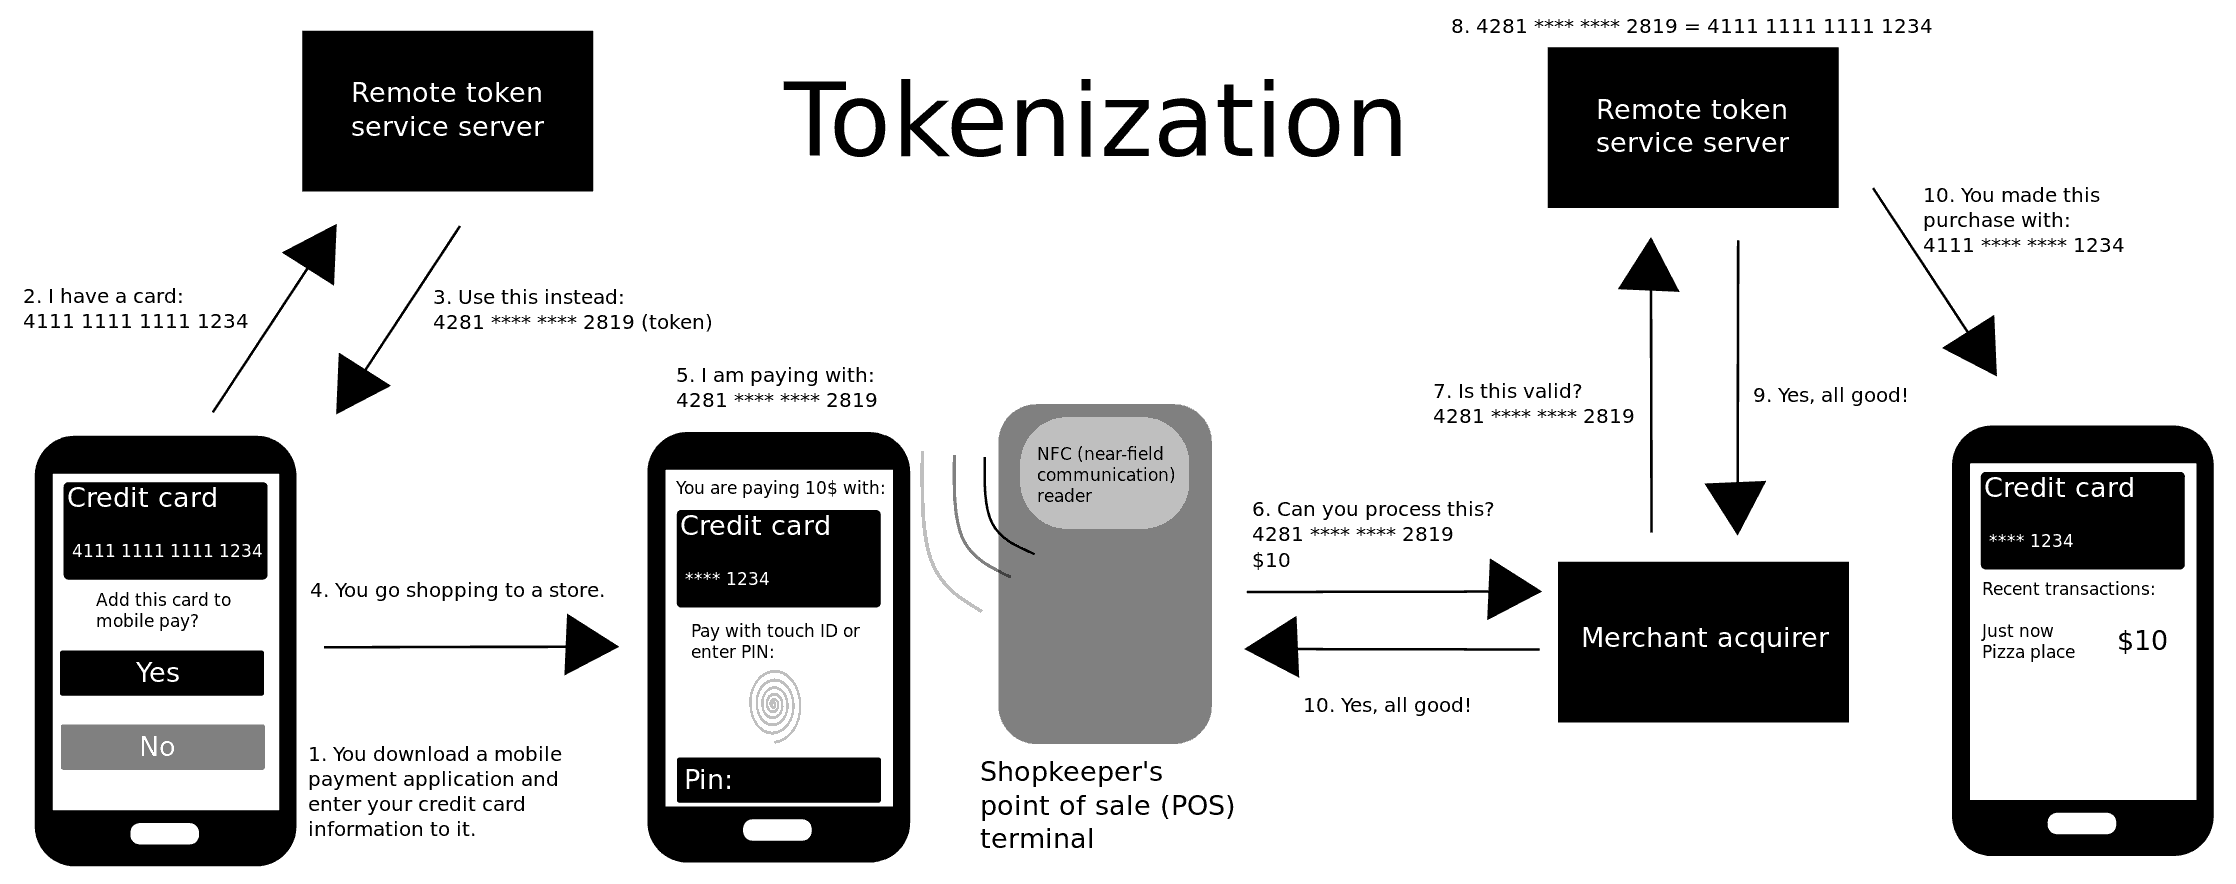
\includegraphics[width=\linewidth]
	{img/Tokenization}
	\caption{Flow van een mobiele betalingsapplicatie met tokenisatie}
	\label{fig:Tokenization}
\end{figure}


\section{Beveiliging op software en hardware niveau}

\subsection{Security Frameworks/Trusted Execution Environment}
\label{subsec:TEE}
Trusted Execution Environment (TEE) is een veilige plaats in de hoofd processor of coprocessor van het toestel waar data kan opgeslagen en verwerkt worden. De bedoeling van een TEE is het uitvoeren van geautoriseerde beveiligingssoftware in een vertrouwde omgeving. TEE bestaat niet enkel uit software maar ook uit hardware die bescherming bieden tegen aanvallen vanuit het besturingssysteem in het toestel. Gevoelige applicaties die beschermd moeten worden tegen het besturingssysteem van het toestel worden opgeslagen in de TEE en helpt ook bij de controle van toegangsrechten tot de applicaties. TEE heeft zijn eigen besturingssysteem, hierdoor kan de TEE niet aangetast worden wanneer het besturingssysteem van het toestel aangetast is. De TEE kan voor een extra beveiligingslaag zorgen voor HCE applicaties ~\autocite{SCA2014}:

\begin{itemize}
	\item \textbf{PIN/wachtwoord ingave.} De TEE kan extra bescherming aanbieden aan de hand van het invoeren van een PIN-code of een wachtwoord. Bij de TEE is de invoer van de PIN-code of een wachtwoord volledig gescheiden van de invoer van het toestel, hierdoor kan de invoer niet onderschept worden door malware applicaties die zich op het besturingssysteem van het toestel bevinden.
	
	\item \textbf{Secure storage of credentials.} De TEE implementeert cryptografische operaties binnen de secure execution environment en zorgt voor het veilig opslaan van sleutels. Hierin kunnen dus tokens/sleutels van betalingsapplicaties in opgeslagen worden, zo zijn deze beter beveiligd tegen aanvallen dan wanneer ze opgeslagen worden in het besturingssysteem van het toestel.
	
	\item \textbf{Secure transfer protocol endpoint.} Het is mogelijk om in de TEE een geëncrypteerd beveiligd kanaal op te zetten aan de kant van de terminal. Dit betekent dat de APDU's geëncrypteerd verstuurd kunnen worden van de terminal en de HCE applicatie via een draadloze interface naar de TEE. Een tweede geëncrypteerd beveiligd kanaal kan opgezet worden tussen de TEE en een Cloud applicatie. Hierdoor zijn de sleutels en data enkel zichtbaar binnen de vertrouwde applicatie, dit biedt een hoger niveau van beveiliging aan dan wanneer de applicatie uitgevoerd zou worden op het besturingssysteem van het toestel.
\end{itemize}



